\section{Removing Edges}
\label{sect:removing-edges}

Similarly, clusters can grow apart and we may want to remove edges between clusters in the cluster graph.
This, too, is not allowed on the inside of the graph, as doing so would create holes and violate the graph's internal triangulatedness. We can only remove edges that lie on the outer face of the cluster graph. Even then, we must ensure that the graph remains $2$-connected. Removing an edge $\{u,w\}$ on the outer face is therefore only permitted if both $u$ and $w$ have degree $d(\cdot) \geq 3$. \cref{fig:remove-outer-edge-example} illustrates a valid edge removal.

\begin{figure}[H]
	\centering
	\subfigure[]{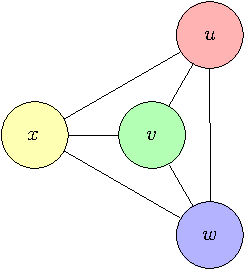
\includegraphics[height=29mm]{Resources/RemoveOuterEdge-Example-1.pdf}}
	\quad
	\subfigure[]{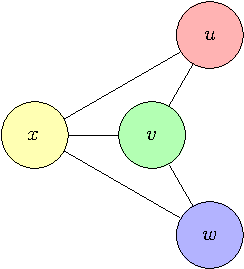
\includegraphics[height=29mm]{Resources/RemoveOuterEdge-Example-2.pdf}}
	\qquad
	\subfigure[]{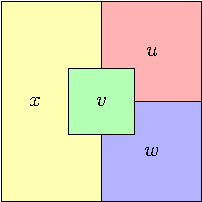
\includegraphics[height=29mm]{Resources/RemoveOuterEdge-Example-3.pdf}}
	\quad
	\subfigure[]{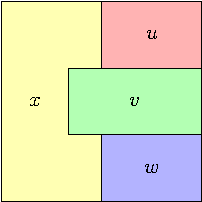
\includegraphics[height=29mm]{Resources/RemoveOuterEdge-Example-4.pdf}}
	\caption{A cluster graph and a polygonal dual thereof, before (a, b) and after (c, d) removing the edge $\{u,w\}$.}
	\label{fig:remove-outer-edge-example}
\end{figure}

\lipsum
